
\chapter{Initial exploration}
\label{cha:1}
In this chapter an initial exploration of the problem is done. This was done in MATLAB with the neural network toolbox for the backpropagation algorithm, and YALMIP with fmincon for the simultaneous approach.

TODO version numbers, hardware

\section{First experiment}
The first experiment conducted was to apply both algorithms to a test problem. A small neural network is constructed with 2 hidden layers with each layer containing 3 nodes with tansig activation function. The activation function was chosen because it works well for a small network. This network is then trained to approximate a piece of a sine function. Both algorithms are trained for 100 epochs. Figure \ref{} shows the training performance for a training run of each algorithm. Both perform well, but the simultaneous approach is much slower. This can be due to the fact that the new algorithm is not well optimized.

\begin{figure}
     \centering
     \begin{subfigure}[b]{0.8\textwidth}
         \centering
         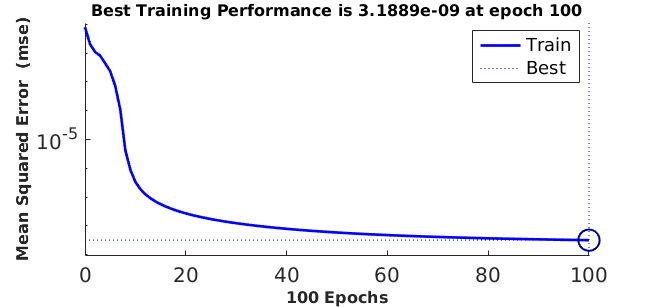
\includegraphics[width=\textwidth]{back_test_1}
         \caption{Training performance of backpropagation}
         \label{fig:y equals x}
     \end{subfigure}
     \begin{subfigure}[b]{0.8\textwidth}
         \centering
         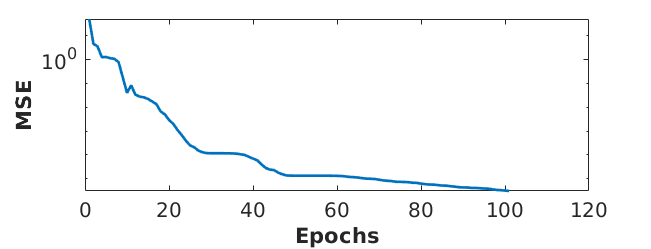
\includegraphics[width=\textwidth]{back_test_12}
         \caption{Training performance of simultaneous approach}
         \label{}
     \end{subfigure}
     \begin{subfigure}[b]{0.8\textwidth}
         \centering
         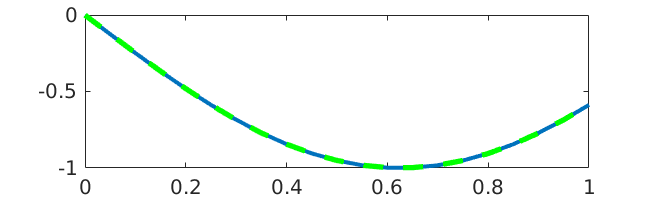
\includegraphics[width=\textwidth]{sine}
         \caption{Sine function}
         \label{}
     \end{subfigure}
        \caption{Performance of algorithms for simple regression problem}
        \label{fig:three graphs}
\end{figure}




The backpropagation algorithm converges every time for this problem, taking anywhere between 10 and 1000 iterations. The stopping criteria is that the validation error increases for 6 consecutive iterations.

The simultaneous approach also converges if the intial conditions are set correctly. The weight variables are randomly initialized and the state variables are initialized by simulating the network once using the input vector, so the initial point is feasible. Letting fmincon run for 200 iterations gives a good solution every time, but the algorithm runs much slower. Its not known if this is due to the difference in optimization of the algorithms and the fact that the backpropagation algorithm is running on my GPU instead of the CPU.

\section{Second experiment}
TODO make it more scientific.

For this experiment the same test problem is considered but with a different network. Here a shallow network 1 layer deep and 10 neurons wide is considered, with the ReLU activation function.

The backpropagation function will sometimes get stuck in a bad solution while training this network, but usually finds a good approximation.

For the simultaneous approach the RELU constraints will have to be reformulated. The ReLU function can be transformed into smooth constraints as follows:

   \begin{gather*}
   x_{k+1}^j = \max(W_kx_k^j,0) \\
   \Updownarrow \\
   x_{k+1}^j = -\min(-W_kx_k^j,0) \\
   \Updownarrow \\
   \min(x_{k+1}^j-W_kx_k^j) = 0 \\
   \Updownarrow \\
   (x_{k+1}^j-W_kx_k^j)^\top x_{k+1}^j = 0,\\
   x_{k+1}^j\geq 0,x_{k+1}^j-W_kx_k^j\geq 0
   \end{gather*}
   
Even using these smooth constraints, the algorithm very often gets stuck in a bad local minimum.
\section{Further exploration}
There are many options that can be explored to further compare these algorithms.

\begin{itemize}
\item Activation function: ReLU is the most popular activation function in the field. Others are tansig, sigmoid, SoftPlus, leaky ReLU, etc.
\item Network size: Networks can be up to thousands of neurons wide and hundreds of layers deep. 
\item Network architecture: There is a huge variety of possible network architectures. Convolutional neural networks for example are very popular for image recognition.
\item Test problems: Neural networks have many applications. Some applications could benefit more from this training method than others.
\item Optimization algorithm: fmincon is quite a general method, a more specific method might perform better
\item Stopping criteria and initial conditions

These will be explored in the next chapters

\end{itemize}




%%% Local Variables: 
%%% mode: latex
%%% TeX-master: "thesis"
%%% End: 
